\documentclass{article}


\usepackage{arxiv}

\usepackage[utf8]{inputenc} % allow utf-8 input
\usepackage[T1]{fontenc}    % use 8-bit T1 fonts
\usepackage{hyperref}       % hyperlinks
\usepackage{url}            % simple URL typesetting
\usepackage{booktabs}       % professional-quality tables
\usepackage{amsfonts}       % blackboard math symbols
\usepackage{nicefrac}       % compact symbols for 1/2, etc.
\usepackage{microtype}      % microtypography
\usepackage{lipsum}
\usepackage{graphics,graphicx}

\title{Using Python to Compare Models and Plot Particle Distribution Following the Lagrangian Flow Network}


\author{
  Jessica Stevens \\
  Ocean, Coastal, and Earth Sciences MS program\\
  University of Texas - Rio Grande Valley\\
  Brownsville, TX 78500 \\
  \texttt{jessica.stevens01@utrgv.edu} \\
  %% examples of more authors
  %% \And
 %%Elias D.~Striatum \\
  %%Department of Electrical Engineering\\
  %%Mount-Sheikh University\\
  %%Santa Narimana, Levand \\
  %%\texttt{stariate@ee.mount-sheikh.edu} \\
  %% \AND
  %% Coauthor \\
  %% Affiliation \\
  %% Address \\
  %% \texttt{email} \\
  %% \And
  %% Coauthor \\
  %% Affiliation \\
  %% Address \\
  %% \texttt{email} \\
  %% \And
  %% Coauthor \\
  %% Affiliation \\
  %% Address \\
  %% \texttt{email} \\
}

\begin{document}
\maketitle

\begin{abstract}
Transport, dispersal, and connectivity within and outside of the Gulf of Mexico (GoM) due to the effects of the Loop Currents (LC) is of particular interest, especially after the Deepwater Horizon oil spill. This research will include the use of Network Theory and Lagrangian oceanographic modeling (Lagrangian Flow Networks, LFN) along with self-organizing maps to assess ocean climate states. The analysis intercompares models to support the Lagrangian patterns that have been observed in our preliminary results. The relevance of this research connects to societally and economically relevant processes, such as pollutant transport, biological transport and connectivity, and retention processes leading to harmful algal blooms. Python will be used to make plots between different model outputs for said intercomparing. 
\end{abstract}


% keywords can be removed
\keywords{lagrangian \and dispersal \and python}


\section{Introduction}
\paragraph{} The loop current in the Gulf of Mexico is a very important oceanic process to understand. Warm, tropical waters enter the Gulf through the Yucatan Chanel. From here the water can either have a quick exit around the Straits of Florida or it protrudes deep into the Gulf then curves down along the Western shelf of Florida to exit and follow the Gulf Stream (Figure 1, Broadus, LaMourie, & Geyer, 2013). As this warm, tropical water enters the Gulf, it occasionally has eddies spin off of it. These eddies can entrap particles, such as nutrients, phytoplankton, and other such small, non-motile organisms (Sebille, et al., 2017). This makes for an interesting biology study in many ways. Given spawning sites of mesophotic corals, for example, the Loop Current and its eddies would need to be understood in order to determine connectivity between sites. In events such as the Deepwater Horizon oil spill, it was one of these eddies that trapped the oil in its spin and carried it away from Florida. We will use Lagrangian (water-following) transport methods to examine the movement of particles in the Gulf of Mexico throughout different LC states: 1) retracted, where the LC barely penetrates the GoM, and the connection between the Yucatan and Florida Currents is short, 2) extended, where the LC extends north, up to the Texas-Louisiana shelf break, bringing Caribbean waters into the GoM, and 3) detached, a transitional state where the LC releases an anti-cyclonic warm-core eddy containing Caribbean waters that then travels westward within the GoM.


\section{Objective}
\label{sec:headings}
\paragraph{}
Firstly, I need to determine if the HYCOM and GECKO data correlates with each other when observing sea surface height and velocities. If there is correlation there, then I will compare these figures with those from Weisberg et al. shown in Figure 2 (Weisberg & Liu, 2017).
\paragraph{} 
Secondly, I will run the LFN code to produce particle distribution and analyze the connectivity between the previous models and this model output.
\paragraph{}
Thirdly, I will attempt to determine if there are patterns of connectivity in the Gulf of Mexico due to the Loop Current.

\section{Methods}
\paragraph{}
Using the Gulf of Mexico Reanalysis data provided by HYCOM online, I will import these netCDF files into xarray. From here I can plot the preferred data which in this case will be sea surface elevation. I can then use quiver to plot velocity vector arrows onto this surface elevation plot. I will plot one month (minimum) of HYCOM data. The same will be done for the GECKO data. If these models share similar agreements on these variables, I can move on to the next step.
\paragraph{}	
Using previously written code with minor edits, I will run the LFN code to return output of particle distribution over one month (or year). The plotting of this data can be done in many ways. The trac files will be imported using pandas and plotted over the Gulf of Mexico area to show the change in position either by final position or by starting position. Some preliminary plots have been made, but have not been analyzed yet. 


%%\bibliographystyle{unsrt}  
\begin{thebibliography}{1}

\bibitem{kour2014real}
Broadus, J. M., LaMourie, M. J., & Geyer, R. A. (2013, May 1). {\em Gulf of Mexico.} Retrieved November 10, 2019, from https://www.britannica.com/place/Gulf-of-Mexico.
\bibitem{}
Sebille, E. van, Griffies, S. M., Abernathey, R., Adams, T. P., Berloff, P., Biastoch, A., … Zika, J. D. (2017, November 24). {\em Lagrangian ocean analysis: Fundamentals and practices.} Retrieved November 10, 2019, from https://www.sciencedirect.com/science/article/pii/S1463500317301853.
\bibitem{}
Weisberg, R. H., & Liu, Y. (2017). {\em On the Loop Current Penetration into the Gulf of Mexico: GULF OF MEXICO LOOP CURRENT PENETRATION.} Journal of Geophysical Research: Oceans, 122(12), 9679–9694. https://doi.org/10.1002/2017JC013330


\end{thebibliography}


\section{Timeline}
\paragraph{}11/10/19 – Submit Proposal
\paragraph{}11/11-17/19 – Plot HYCOM and GECKO data, make movie for comparison
\paragraph{}11/18-24/19 – Run LFN code and make plots.
\paragraph{}11/25-12/1/19 – Compare all of the output and make presentation
\paragraph{}12/2-8/19 – Write Final Paper, Present
\paragraph{}12/11/19 – Make sure I’ve submitted final paper
\paragraph{} 



\section{Figures}

\begin{figure}
    \centering
    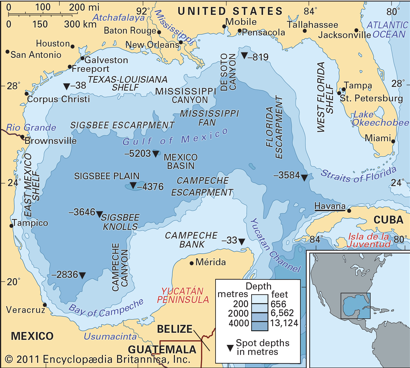
\includegraphics{Picture1.png}
    \caption{A detailed image of the Gulf of Mexico (Broadus, LaMourie, & Geyer, 2013)}
    \label{fig:my_label}
\end{figure}

\begin{figure}
    \centering
    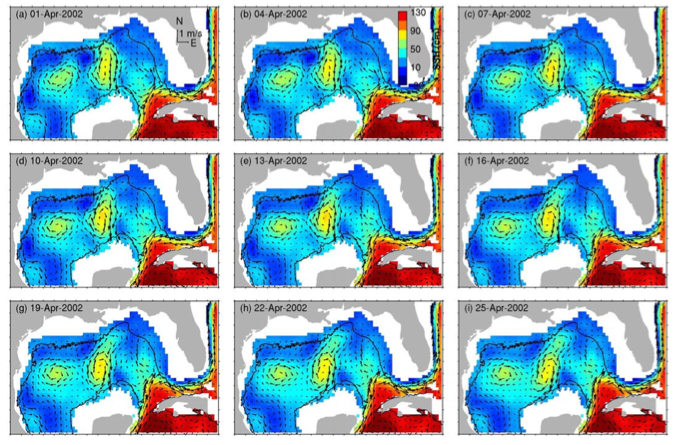
\includegraphics{Picture2.png}
    \caption{This figure shows one month of the Loop Current state in the Gulf of Mexico. This will be a basis of comparison for the other models. (Weisberg & Liu, 2017).}
    \label{fig:my_label}
\end{figure}



\end{document}
